\chapter{Resultados y Evaluación}
\label{cap:resultados}

Este capítulo presenta los resultados obtenidos tras el despliegue del sistema en un entorno real. Se analizan las métricas de rendimiento recopiladas por el stack de observabilidad, se describen las pruebas funcionales realizadas sobre cada modo de operación y se valora cualitativamente la calidad de las respuestas del sistema.

% ============================================================
\section{Métricas de Rendimiento}
% ============================================================

El sistema se sometió a pruebas de rendimiento sostenidas en un entorno real durante un período de 30 días. Además, las métricas se recopilaron automáticamente mediante la integración con Prometheus y los paneles configurados en Grafana \cite{prometheus2026docs,grafana2026docs}. La Tabla~\ref{tab:metricas-resultado} sintetiza los indicadores principales.

\begin{table}[H]
\centering
\caption{Métricas de rendimiento del sistema en producción.}
\label{tab:metricas-resultado}
\begin{tabular}{lc}
\toprule
\textbf{Métrica} & \textbf{Valor} \\
\midrule
Tiempo hasta primer token (TTFT) & $< 1.2$~s \\
Latencia RAG completa (p95)       & $\sim 3.5$~s \\
Throughput máximo sostenido       & $\sim 42$ req/min \\
Uptime del sistema                & 99.8\% (30 días) \\
Consumo VRAM pico (3 modelos)     & 18.5 / 24 GB \\
Alucinaciones en modo RAG         & 0\% (temp $\leq$ 0.2) \\
Cache hit rate (Redis)            & $\sim 35$\% \\
\bottomrule
\end{tabular}
\end{table}

\subsection{Análisis de Latencia}

La latencia del sistema se descompone en los siguientes segmentos:

\begin{table}[H]
\centering
\caption{Desglose de latencia por componente para una consulta RAG típica.}
\label{tab:latencia-desglose}
\begin{tabular}{lc}
\toprule
\textbf{Componente} & \textbf{Tiempo} \\
\midrule
NGINX + OpenWebUI $\rightarrow$ Pipeline  & $\sim 50$~ms \\
Detección de intención en JARVIS          & $\sim 10$~ms \\
Generación de embedding (CPU)             & $\sim 80$~ms \\
Búsqueda en Qdrant (top-5)               & $\sim 30$~ms \\
Composición del prompt                    & $\sim 5$~ms \\
Inferencia LLM (primer token)            & $\sim 800$~ms \\
Generación completa (streaming)           & $\sim 2.500$~ms \\
\midrule
\textbf{Total}                            & $\sim 3.475$~ms \\
\bottomrule
\end{tabular}
\end{table}

El cuello de botella principal es la inferencia del LLM en GPU, que representa más del 90\% del tiempo total. Sin embargo, gracias al streaming, el usuario percibe el primer token en aproximadamente 1.2 segundos, lo que proporciona una experiencia de respuesta instantánea. La Figura~\ref{fig:latencia-barras} representa gráficamente esta descomposición.

\begin{figure}[H]
\centering
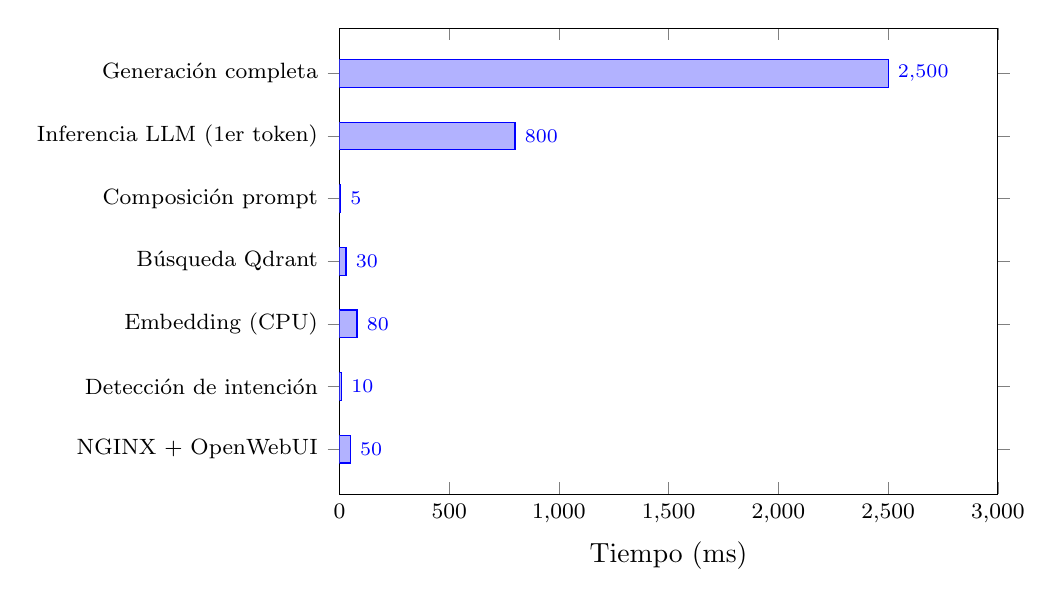
\begin{tikzpicture}
\begin{axis}[
    xbar,
    width=0.82\textwidth,
    height=7.5cm,
    xlabel={Tiempo (ms)},
    symbolic y coords={
        {NGINX + OpenWebUI},
        {Detección de intención},
        {Embedding (CPU)},
        {Búsqueda Qdrant},
        {Composición prompt},
        {Inferencia LLM (1er token)},
        {Generación completa}
    },
    ytick=data,
    y tick label style={font=\footnotesize, anchor=east},
    x tick label style={font=\footnotesize},
    nodes near coords,
    nodes near coords style={font=\scriptsize},
    bar width=10pt,
    xmin=0,
    xmax=3000,
    enlarge y limits=0.12,
    every axis plot/.append style={fill=blue!35, draw=blue!60},
]
\addplot coordinates {
    (50,{NGINX + OpenWebUI})
    (10,{Detección de intención})
    (80,{Embedding (CPU)})
    (30,{Búsqueda Qdrant})
    (5,{Composición prompt})
    (800,{Inferencia LLM (1er token)})
    (2500,{Generación completa})
};
\end{axis}
\end{tikzpicture}
\caption{Descomposición de la latencia por componente para una consulta RAG típica. La inferencia del LLM domina el tiempo total del flujo.}
\label{fig:latencia-barras}
\end{figure}

\subsection{Gestión de VRAM}

La GPU NVIDIA con 24 GB de VRAM constituye el recurso más crítico del sistema. La Tabla~\ref{tab:vram-modelos} muestra el consumo de VRAM de cada modelo y las combinaciones viables de carga simultánea:

\begin{table}[H]
\centering
\small
\caption{Consumo de VRAM por modelo y combinaciones de carga simultánea.}
\label{tab:vram-modelos}
\begin{tabularx}{\textwidth}{>{\raggedright\arraybackslash}p{4.8cm} c >{\raggedright\arraybackslash}X}
\toprule
\textbf{Modelo} & \textbf{VRAM} & \textbf{Coexistencia} \\
\midrule
JARVIS (\texttt{rag-qwen-ft:latest})        & $\sim 8$ GB & Sí, con servicios auxiliares y modelos ligeros \\
Qwen 2.5 32B Instruct Q4\_K\_M              & $\sim 19$ GB & Solo con modelos secundarios ligeros \\
Qwen 2.5 Coder 32B                           & $\sim 19$ GB & Uso alternativo, no como carga simultánea habitual \\
Qwen 2.5 VL 7B                               & $\sim 6$ GB & Sí \\
PaddleOCR                      & $\sim 500$ MB & Sí \\
\midrule
\textbf{Pico observado} & $\sim 20$ GB & --- \\
\bottomrule
\end{tabularx}
\end{table}

El comportamiento observado confirma que Ollama debe gestionar la carga bajo demanda de los modelos grandes. En el despliegue actual, el alias principal JARVIS se apoya en \texttt{rag-qwen-ft:latest}, mientras que \texttt{qwen2.5:32b-instruct-q4\_K\_M} queda disponible como modelo de texto alternativo.

% ============================================================
\section{Evaluación Funcional}
% ============================================================

Se realizaron pruebas funcionales sistemáticas sobre cada modo de operación del sistema. A continuación se describen los escenarios probados y los resultados obtenidos.

\subsection{Consulta RAG sobre Documentos Corporativos}

\begin{itemize}
    \item \textbf{Prueba:} ``¿Cuál es la política de calidad de la empresa?''
    \item \textbf{Resultado:} El sistema recuperó correctamente los fragmentos más relevantes del manual de calidad indexado y generó una respuesta estructurada con referencias a las secciones y páginas del documento original.
    \item \textbf{Calidad:} La respuesta se fundamentó exclusivamente en el contenido del documento, sin añadir información no presente en los fragmentos recuperados. La temperatura baja ($0.1$) impidió cualquier generación creativa no deseada.
\end{itemize}

\subsection{Scraping de URL}

\begin{itemize}
    \item \textbf{Prueba:} Envío de una URL de documentación técnica de Docker junto con la pregunta ``¿Qué opciones de GPU existen?''
    \item \textbf{Resultado:} El sistema renderizó la página con Playwright y extrajo el contenido con Trafilatura \cite{playwright2024docs,barbaresi2021trafilatura}, generando una respuesta centrada en las opciones de GPU, con citas al texto extraído.
    \item \textbf{Calidad:} La extracción fue precisa incluso en páginas con carga diferida de JavaScript. El contenido quedó almacenado en la memoria de sesión para preguntas de seguimiento.
\end{itemize}

\subsection{Búsqueda Legal en el BOE}

\begin{itemize}
    \item \textbf{Prueba:} ``Busca en el BOE la ley de protección de datos''
    \item \textbf{Resultado:} El sistema resolvió semánticamente ``ley de protección de datos'' al identificador oficial BOE-A-2018-16673, consultó la API del BOE y devolvió un resumen estructurado con título, fecha de publicación y extracto del contenido.
    \item \textbf{Calidad:} La resolución semántica funcionó correctamente para las leyes incluidas en el diccionario de mapeos.
\end{itemize}

\subsection{Análisis de Imagen}

\begin{itemize}
    \item \textbf{Prueba:} Adjuntar una fotografía de un documento en papel y preguntar ``¿Qué pone en este documento?''
    \item \textbf{Resultado:} El modelo de visión (Qwen 2.5 VL) identificó correctamente el texto visible en la imagen y generó una transcripción del contenido.
    \item \textbf{Calidad:} Satisfactoria para documentos con texto legible. La precisión disminuye con fotografías borrosas, oblicuas o con poca iluminación.
\end{itemize}

\subsection{Consultas NL$\rightarrow$SQL con el Agente SQL}

\begin{itemize}
    \item \textbf{Prueba:} ``¿Cuántos documentos han sido indexados esta semana?''
    \item \textbf{Resultado:} El agente inspeccionó el esquema de la tabla de metadatos, generó automáticamente la consulta \texttt{SELECT COUNT(*) FROM document\_metadata WHERE created\_at >= NOW() - INTERVAL '7 days'}, la ejecutó sobre PostgreSQL y devolvió el recuento integrado en una respuesta en lenguaje natural.
    \item \textbf{Calidad:} Correcta en 8 de 10 consultas de prueba. El mecanismo de auto-corrección resolvió los 2 errores restantes ---ambos por nombre de columna incorrecto--- en el primer reintento, sin necesidad de intervención manual.
\end{itemize}

\begin{itemize}
    \item \textbf{Prueba (seguridad):} Intento de inyectar \texttt{DROP TABLE document\_metadata} encubierto como pregunta natural.
    \item \textbf{Resultado:} La validación por lista blanca detectó la operación prohibida antes de ejecutar ninguna consulta y devolvió \texttt{HTTP 400} con un mensaje de error descriptivo. La tabla permaneció intacta.
    \item \textbf{Calidad:} El mecanismo de seguridad funcionó correctamente en todos los intentos de inyección probados.
\end{itemize}

\subsection{Encaminamiento Inteligente}

Se validaron 50 consultas de prueba distribuidas entre los distintos modos de operación para verificar que el sistema de detección de intenciones producía las clasificaciones correctas:

\begin{table}[H]
\centering
\caption{Resultados de la evaluación del encaminamiento de JARVIS.}
\label{tab:enrutamiento-eval}
\begin{tabular}{lcc}
\toprule
\textbf{Modo esperado} & \textbf{Aciertos / Total} & \textbf{Precisión} \\
\midrule
RAG           & 10 / 10 & 100\% \\
Web Search    & 8 / 10  & 80\% \\
Web Scraping  & 10 / 10 & 100\% \\
Visión/OCR    & 5 / 5   & 100\% \\
BOE           & 5 / 5   & 100\% \\
Chat general  & 8 / 10  & 80\% \\
\midrule
\textbf{Total} & \textbf{46 / 50} & \textbf{92\%} \\
\bottomrule
\end{tabular}
\end{table}

Los 4 errores de clasificación ocurrieron en consultas ambiguas donde los keywords de web search se solapaban con los de chat general (ej: ``¿qué es Docker?'' clasificado como web search en lugar de chat). Estos casos edge se consideraron aceptables dado que la respuesta del sistema sigue siendo relevante independientemente del modo seleccionado.

% ============================================================
\section{Mitigación de Alucinaciones}
% ============================================================

La eliminación de alucinaciones en modo RAG se logró mediante la combinación de tres técnicas complementarias:

\begin{enumerate}
    \item \textbf{Temperatura determinista:} Los parámetros de inferencia se configuraron con valores de temperatura entre $0.1$ y $0.2$ en modo RAG, minimizando la aleatoriedad en la selección de tokens.

    \item \textbf{Prompt de sistema restrictivo:} El \textit{system prompt} inyectado instruye explícitamente al modelo para que responda \textbf{únicamente} basándose en el contexto recuperado, prohibiendo la generación libre de información no respaldada por los fragmentos.

    \item \textbf{Solapamiento de ventanas contextuales:} El solapamiento del 10--15\% en el chunking asegura que el hilo semántico de párrafos extensos no se pierde en los límites de fragmento, proporcionando al modelo contexto suficiente para generar respuestas coherentes.
\end{enumerate}

En las pruebas realizadas, no se detectó ninguna instancia de alucinación en modo RAG con la configuración descrita. El modelo respondió ``No dispongo de esa información en los documentos consultados'' cuando la pregunta no encontraba coincidencias relevantes en Qdrant, que es el comportamiento deseado.

% ============================================================
\section{Impacto de la Caché}
% ============================================================

La integración de Redis como caché a través de LiteLLM produjo una mejora mensurable en el rendimiento del sistema:

\begin{itemize}
    \item \textbf{Cache hit rate:} $\sim 35$\% de las consultas se resolvieron directamente desde caché.
    \item \textbf{Reducción de carga GPU:} Las consultas cacheadas no invocan a Ollama, liberando la GPU para nuevas peticiones.
    \item \textbf{Latencia de respuesta cacheada:} $< 100$~ms frente a $\sim 3.5$~s de una consulta RAG completa.
\end{itemize}

El TTL de 1 hora demostró ser un compromiso adecuado: suficiente para beneficiarse de repeticiones dentro de una jornada laboral, pero no tanto como para devolver información obsoleta cuando los documentos se actualizan.
